\documentclass[10pt,twocolumn,letterpaper]{article}

\usepackage{cvpr}
\usepackage{times}
\usepackage{epsfig}
\usepackage{graphicx}
\usepackage{amsmath}
\usepackage{amssymb}
\usepackage{enumerate}
\usepackage{graphicx}

% Include other packages here, before hyperref.

% If you comment hyperref and then uncomment it, you should delete
% egpaper.aux before re-running latex.  (Or just hit 'q' on the first latex
% run, let it finish, and you should be clear).
\usepackage[breaklinks=true,bookmarks=false]{hyperref}

\cvprfinalcopy % *** Uncomment this line for the final submission

\def\cvprPaperID{****} % *** Enter the CVPR Paper ID here
\def\httilde{\mbox{\tt\raisebox{-.5ex}{\symbol{126}}}}

% Pages are numbered in submission mode, and unnumbered in camera-ready
%\ifcvprfinal\pagestyle{empty}\fi
\setcounter{page}{1}
\begin{document}

%%%%%%%%% TITLE
\title{EECS 442 Computer Vision: Final Project Progress Report}

\author{Nathan Immerman\\
College of Engineering, University of Michigan\\
Ann Arbor, Michigan\\
{\tt\small immerman@umich.edu}
% For a paper whose authors are all at the same institution,
% omit the following lines up until the closing ``}''.
% Additional authors and addresses can be added with ``\and'',
% just like the second author.
% To save space, use either the email address or home page, not both
\and
Alexander Chocron\\
College of Engineering, University of Michigan\\
Ann Arbor, Michigan\\
{\tt\small achocron@umich.edu}
}

\maketitle
%\thispagestyle{empty}

%%%%%%%%% BODY TEXT
\section{Introduction}
Our project is to implement the algorithm outlined by Johnson and Farid's paper "Exposing Digital Forgeries by Detecting Inconsistencies in Lighting"  [1]. This algorithm is able to detect artificially composited images by determining whether the components are consistently lit. We will present this application as a MATLAB Graphical User Interface application that will take user input, decide whether the image is a forgery, and display the computed light directions on the objects specified by the user.

%------------------------------------------------------------------------
\section{Work Accomplished}
 We have written the code to collect occluding boundaries of objects in the image, partition these boundaries into patches,  find the normal vectors of these patches, and extrapolate the intensity of the occluding pixels at these patches. We have also begun to create a GUI that will stitch all of the pieces together. 

 In accordance with the method described in the paper, we determined the best way to collect the occluding boundaries of objects is through user input. As of now, the GUI displays the image in question and allows a user to draw the various relevant boundaries on the image itself (Figure 1). 

\begin{figure}[]
\centering
 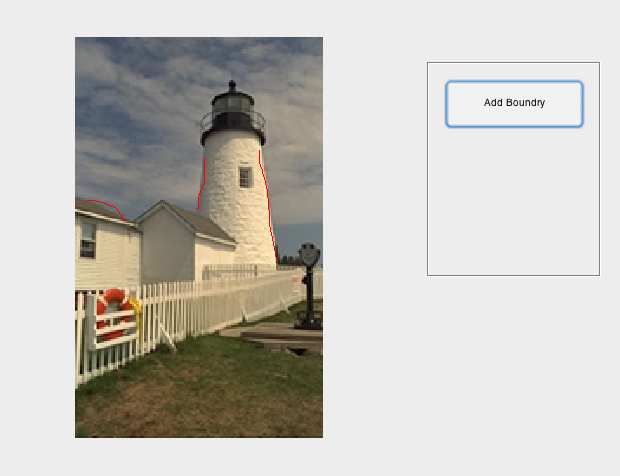
\includegraphics[scale=0.35]{gui_pic.png}
\caption{Current State of our GUI, user selected boundaries in red}
\end{figure}

 Once the boundaries are collected, they are partitioned into about eight patches. This partitioning function has been implemented. To estimate the normal vectors for each patch, we are going need to collect three user entered points for each patch (not implemented yet) and then fit a quadratic curve to estimate the contour of the patch which can then be used to estimate the normal vectors (implemented). We can then use the normals to fit a power function to the pixels along the normal direction on the object to estimate the intensities of the occluding pixels (implemented). At a certain point in the algorithm, we need to calculate a matrix $C$ as a function of the number of partitions and the size of each partition (implemented). At this point we have coded but not tested the mechanisms to collect almost all of the information that we need to be able to run the algorithm described in the paper.
%------------------------------------------------------------------------
\section{Work to be Done}

We have accomplished a significant portion of our algorithm, but we still have many tasks to complete. All of our implemented code is untested as of yet. This is because testing requires more code to be completed - we must implement another function that takes all of the outputs from our existing functions and runs the algorithm in completion. We are unable to test our existing functions without the proper input, and this means that we must complete the other input portions of our GUI. We must then test all of our code, and fix any bugs we find. The code we have already written is for detecting inconsistencies in lighting assuming an infinite light source, but we also must implement code that detects inconsistencies assuming a local light source. Though some of our functions will be applicable to this problem, we will also need to write additional code. This includes implementing or finding an implementation of conjugate gradient descent. CGD is necessary because the local light source least squares error minimization has no closed form solution and must be solved iteratively. We will also need to update our GUI to accommodate this setting.

Lastly, we will need to test everything. We will create test cases by taking pictures both outdoors and indoors with known light sources, and testing how well the algorithm is able to determine the light directions. We will also create composite images in different lighting and determine how well the algorithm is able to distinguish between the two (or more) inconsistent directions.

We would like to point out that while originally we had planned to create an iOS application to demonstrate the algorithm, we have since decided to make a MATLAB GUI instead. We were at first unsure whether MATLAB was capable of providing a robust interface for accepting various types of input that the algorithm requires. Further, making an iOS application would require extensive learning about iOS development whereas both of us are already competent in MATLAB. It would also require converting all of our MATLAB code to c++, which would take time that we would rather spend improving our algorithms and adding features to our GUI.
%------------------------------------------------------------------------
\section{References}

[1] M. K. Johnson and H. Farid. Exposing digital forgeries by detecting inconsistencies in lighting. \emph{In Proceedings of the 7th workshop on Multimedia and security}, pages 1-10, 2005.


\end{document}































